\begin{comment}
\end{comment}

\part{Théorie}\label{part:theory}

\chapter{Verre de spin} \label{ch:spin-glass}
\section{Définition} \label{sec:spin-glass}
De manière générale, les verres de spin sont des états magnétiques qui contiennent $n$ spins qui interagissent ensemble.
L'Hamiltonien le plus simple permettant de décrire un tel système est le suivant:
\begin{equation}
    \mathcal{H} = -\frac{1}{2}\sum_{i,j = 0}^{n-1}J_{ij}\sigma_i\sigma_j,
\end{equation}
où $J_{ij}$ représente le couplage entre les spins $\sigma_i$ et $\sigma_j$ qui peuvent être soit des spins d'Ising ou des spins respectant $||\vec{\sigma}|| = n$ (une contrainte sphérique)~\cite{EAspinglass, spherical-model-spinglass}.
Dans le premier cas, les spins sont tous limités à être des valeurs entre $+1$ et $-1$ tandis que dans le deuxième, ils sont des variables réels.
Dans cette définition du problème, on a évidemment que $J_{ii} = 0$ et que $J_{ij} = J_{ji}$.
Ces systèmes physiques ayant une certaine complexité au niveau structurel, ils peuvent présenter de la \emph{frustration} au niveau des spins ainsi que de la \emph{métastabilité}~\cite{stein2013spin}.
La métastabilité vient du fait que ces systèmes physiques peuvent rester << coincés >> dans une configuration de spins qui n'est pas à l'énergie fondamentale du système, mais plutôt à une énergie qui lui est proche, et le concept de frustration est schématiquement représenté à la figure~\ref{fig:spin-glass-frustration}.
\begin{figure}[h]
    \centering
    \includegraphics[width=0.35\textwidth]{Figures/plaquette.pdf}
    \caption[Un système à quatre spins d'Ising dans lequel les spins interagissent de manière ferromagnétique (avec $J = +1$), excepté pour le couplage du bas.]{Un système à quatre spins de'Ising dans lequel les spins interagissent de manière ferromagnétique (avec $J = +1$), excepté pour le couplage du bas. Cela fait en sorte que le spin en bas à gauche est couplé ferromagnétiquement et antiferromagnétiquement avec les spins au-dessus de lui et à sa droite. Il ne << sait >> donc pas comment il devrait se positionner afin de satisfaire ces deux couplages, donc de minimiser l'énergie. Image tirée de~\protect\cite{altieri2023introduction}.}
    \label{fig:spin-glass-frustration}
\end{figure}
Plusieurs modèles ont été développé afin d'étudier différentes variantes de ce type de système physique, comme le modèle de Sherrington-Kirkpatrick (SK)~\cite{SKspinglass}, le modèle de Edwards-Anderson (EA)~\cite{EAspinglass} et le modèle de la grille de Bethe~\cite{Bethespinglass} pour en nommer quelques-uns. %~\cite{zamponi2010mean}

Le modèle SK est aussi appelé le modèle \emph{complètement connecté} où les spins sont des spins d'Ising.
En effet, celui-ci étudie le cas où chacun des spins est connecté avec tous les autres qui sont présents dans le système soit par un couplage ferromagnétique ou par un couplage antiferromagnétique.
L'Hamiltonien de ce modèle est le suivant:
\begin{equation}
    \mathcal{H} = -\frac{1}{\sqrt{n}}\sum_{i < j} J_{ij}\sigma_i\sigma_j.
\end{equation}
Généralement, ces couplages suivent une probabilité de distribution gaussienne de moyenne $J_0 / n$ et de variance $J^2 / n$~\cite{rodriguez2021sherrington} et le coefficient $1/\sqrt{n}$ est utile au niveau de la normalisation de l'énergie lorsque le système étudié est de grande taille ($n \rightarrow \infty$)~\cite{stein2013spin}.
Quant à lui, le modèle EA, aussi appelé modèle à \emph{dimension finie} (ou à \emph{connexion finie}), est assez similaire au modèle SK, mais à la différence que les spins sont distribués sur une grille de $d$-dimensions et que seulement les plus proches voisins interagissent entre eux~\cite{stein2013spin}.
L'Hamiltonien de ce modèle est:
\begin{equation}
    \mathcal{H} = -\sum_{\langle i, j \rangle} J_{ij}\sigma_i\sigma_j,
\end{equation}
où $\langle i, j \rangle$ correspond à la connexion des spins $\sigma_i$ et $\sigma_j$, deux proches voisins sur la grille.
La plupart du temps, la distribution de probabilité suivie par les $J_{ij}$ est uniforme entre deux valeurs, $+J$ et $-J$\cite{stein2013spin}.
Pour ce qui en est du modèle de la grille de Bethe, celui-ci est aussi semblable aux deux autres, mais les spins y sont organisés sur une grille sur laquelle chacun d'eux possède exactement $z$ voisins~\cite{viana1985phase}.
Un exemple de grille dans ce modèle est une grille de Bethe, montrée à la figure~\ref{fig:bethe-lattice}.
\begin{figure}[h]
    \centering
    \includegraphics[width=0.4\textwidth]{Figures/Reseau_de_Bethe.pdf}
    \caption[Représentation d'un réseau de Bethe avec $z = 3$ voisins.]{Représentation d'un réseau de Bethe, une grille qui a la forme d'un arbre où chacun des sommets possède exactement $z = 3$ voisins. Image libre de droits, tirée de~\protect\cite{wiki:Bethe-lattice}.}
    \label{fig:bethe-lattice}
\end{figure}

% Visuellement, les verres de spin peuvent se représenter sous la forme d'un \emph{graphe}, concept défini à la définition~\ref{def:graph}.
% \begin{definition}\label{def:graph}
%     Un \textbf{graphe} $G = (V, E)$ est un objet mathématique qui correspond à un ensemble de sommets $V$ et d'arêtes $E = \{uv\ |\ u, v \in V\}$. Afin de visualiser le concept, un graphe possédant $|V| = 6$ sommets  et $|E| = 7$ arêtes est représenté à la figure~\ref{fig:random-graph}.
% \end{definition}
% Visuellement, les verres de spin peuvent se représenter sous la forme d'un \emph{graphe} $G = (V, E)$, un objet mathématique qui correspond à un ensemble de sommets $V$ et d'arêtes $E = \{uv\ |\ u, v \in V\}$.
% Afin de visualiser le concept, un graphe possédant $|V| = 6$ sommets  et $|E| = 7$ arêtes est représenté à la figure~\ref{fig:random-graph}.
% \begin{figure}[h]
%     \centering
%     \includegraphics[width=0.65\textwidth]{Figures/graph_example.pdf}
%     \caption{Graphe contenant six sommets $V = \{v_1, v_2, v_3, v_4, v_5, v_6\}$ et sept arêtes $E = \{v_1v_6, v_2v_3, v_2v_6, v_3v_4, v_3v_5, v_4v_5, v_5v_6\}$.}
%     \label{fig:random-graph}
% \end{figure}
% En effet, ce type de système physique peut se modéliser par un graphe $G = (U, V, E)$ où $U$ correspond à l'ensemble de sommets qui représentent les $|U| = n$ spins, $V$ correspond à l'ensemble de sommets qui représentent les $|V| = m$ termes d'interaction entre ces spins et $E$ correspond à l'ensemble d'arêtes qui connectent les sommets de $U$ avec ceux dans $V$.
% La définition de l'ensemble $E$ fait en sorte que les sommets en $U$ ne se connectent qu'avec ceux qui se trouvent en $V$, et vice-versa, ce qui revient à dire qu'il est un graphe \emph{biparti}.

% Originant de la matière condensée, les verres de spin se retrouvent maintenant dans des disciplines qui en sont bien éloignées, comme l'informatique théorique~\cite{kirkpatrick1985configuration}, la biologie~\cite{bryngelson1987spin} et l'apprentissage machine~\cite{venkataraman1991spin}.
Tous les modèles de verres de spin, y compris les trois présentés ci-haut, partagent la même caractéristique: ils présentent des paysages énergétiques ayant une allure << accidentée >>, comme celui montré à la figure~\ref{fig:spin-glass-rugged-energy-landscape}. % ~\cite{stein2013spin}
\begin{figure}[h]
    \centering
    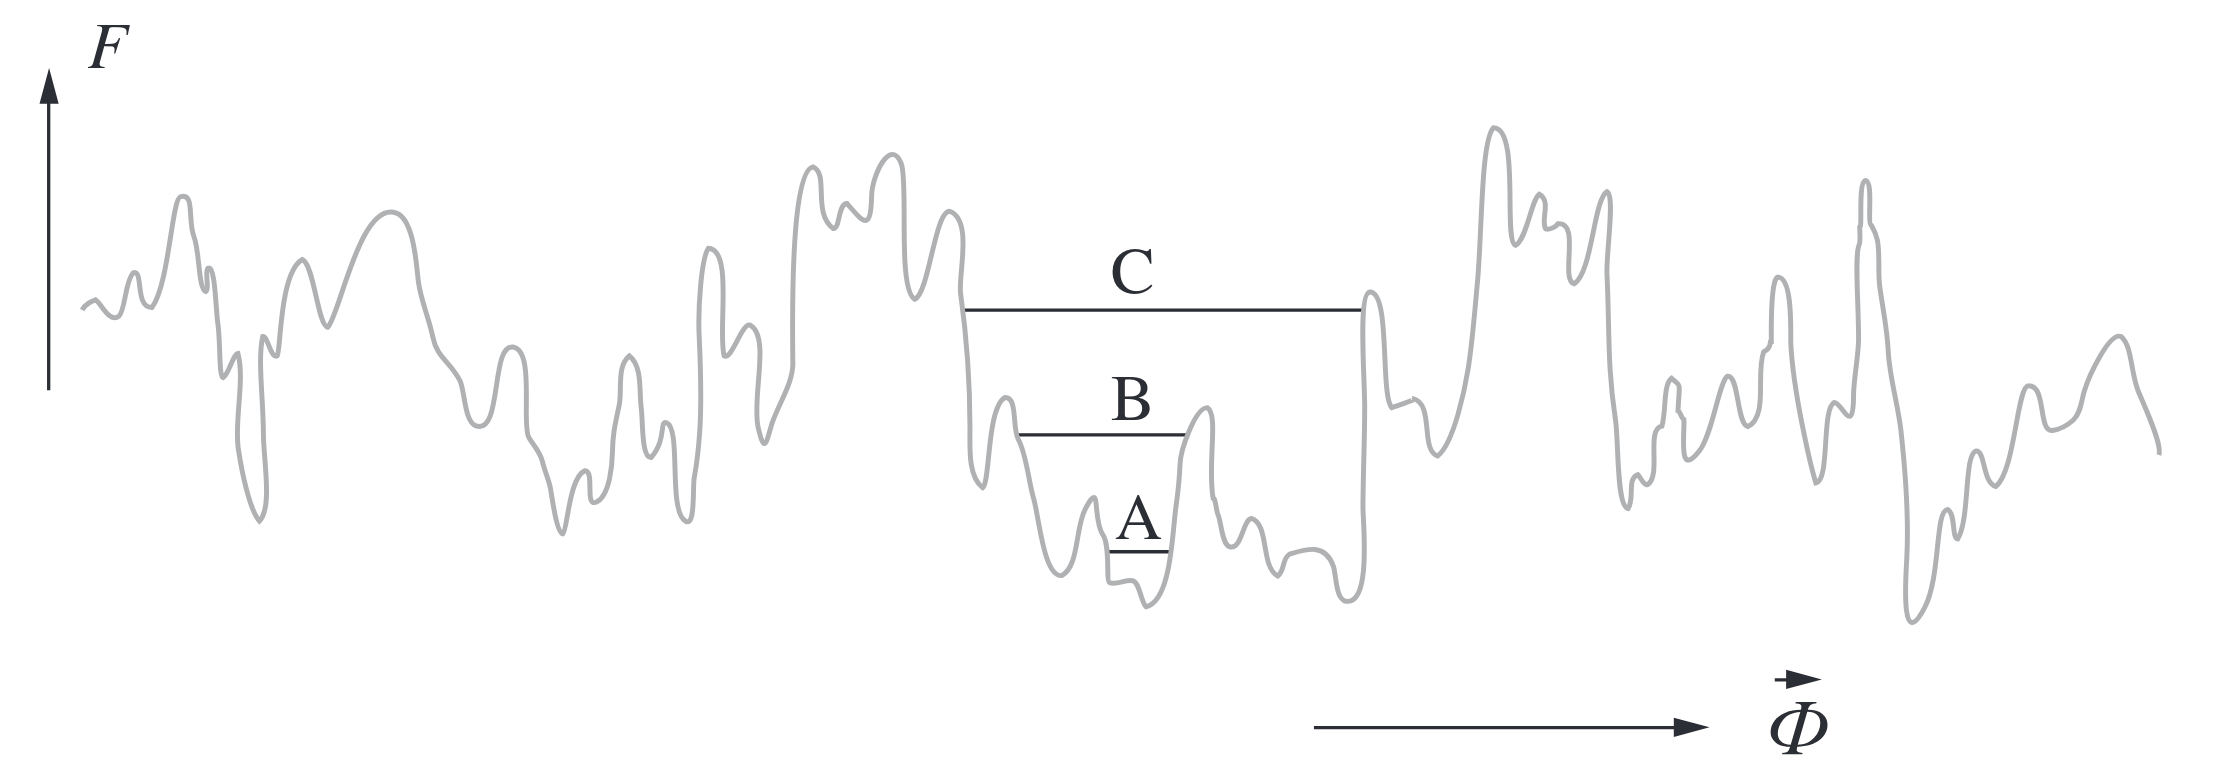
\includegraphics[width=0.9\textwidth]{Figures/spin-glass-rugged-energy-landscape.png}
    \caption[Un exemple de paysage énergétique d'un système de verre de spin.]{Un exemple de paysage énergétique d'un système de verre de spin en fonction des différentes configurations de spins possibles. Image tirée de~\protect\cite{stein2013spin}.}
    % Les multiples minimums locaux font en sorte que les algorithmes prennent du temps à résoudre le problème.
    \label{fig:spin-glass-rugged-energy-landscape}
\end{figure}
Cela fait en sorte que les algorithmes d'optimisation qui tentent de travailler sur ces modèles afin de trouver un état fondamental (ou la fonction de partition) d'un système ont tendance à être piégés dans ces minimums locaux, menant à des temps d'exécution exponentiellement longs.
On peut donc dire que les modèles de verre de spin sont simples à décrire, mais difficiles à résoudre.

% Les modèles pour les verres de spin sont, comme on le voit avec les $3$ modèles brièvement présentés, simple à décrire, mais ils sont toutefois difficiles à résoudre.
% Par résoudre, on entend ici de trouver un état fondamental du système ou d'évaluer sa fonction de partition.
% Une raison de cette difficulté vient du fait que ces modèles présentent des paysages énergétiques aillant une allure << accidentée >>~\cite{stein2013spin}, piégeant les algorithmes d'optimisation dans des minimums locaux et conduisant à des temps d'exécution exponentiellement longs.
% Un exemple de paysage énergétique accidenté est présenté à la figure~\ref{fig:spin-glass-rugged-energy-landscape}.
% \begin{figure}[h]
%     \centering
%     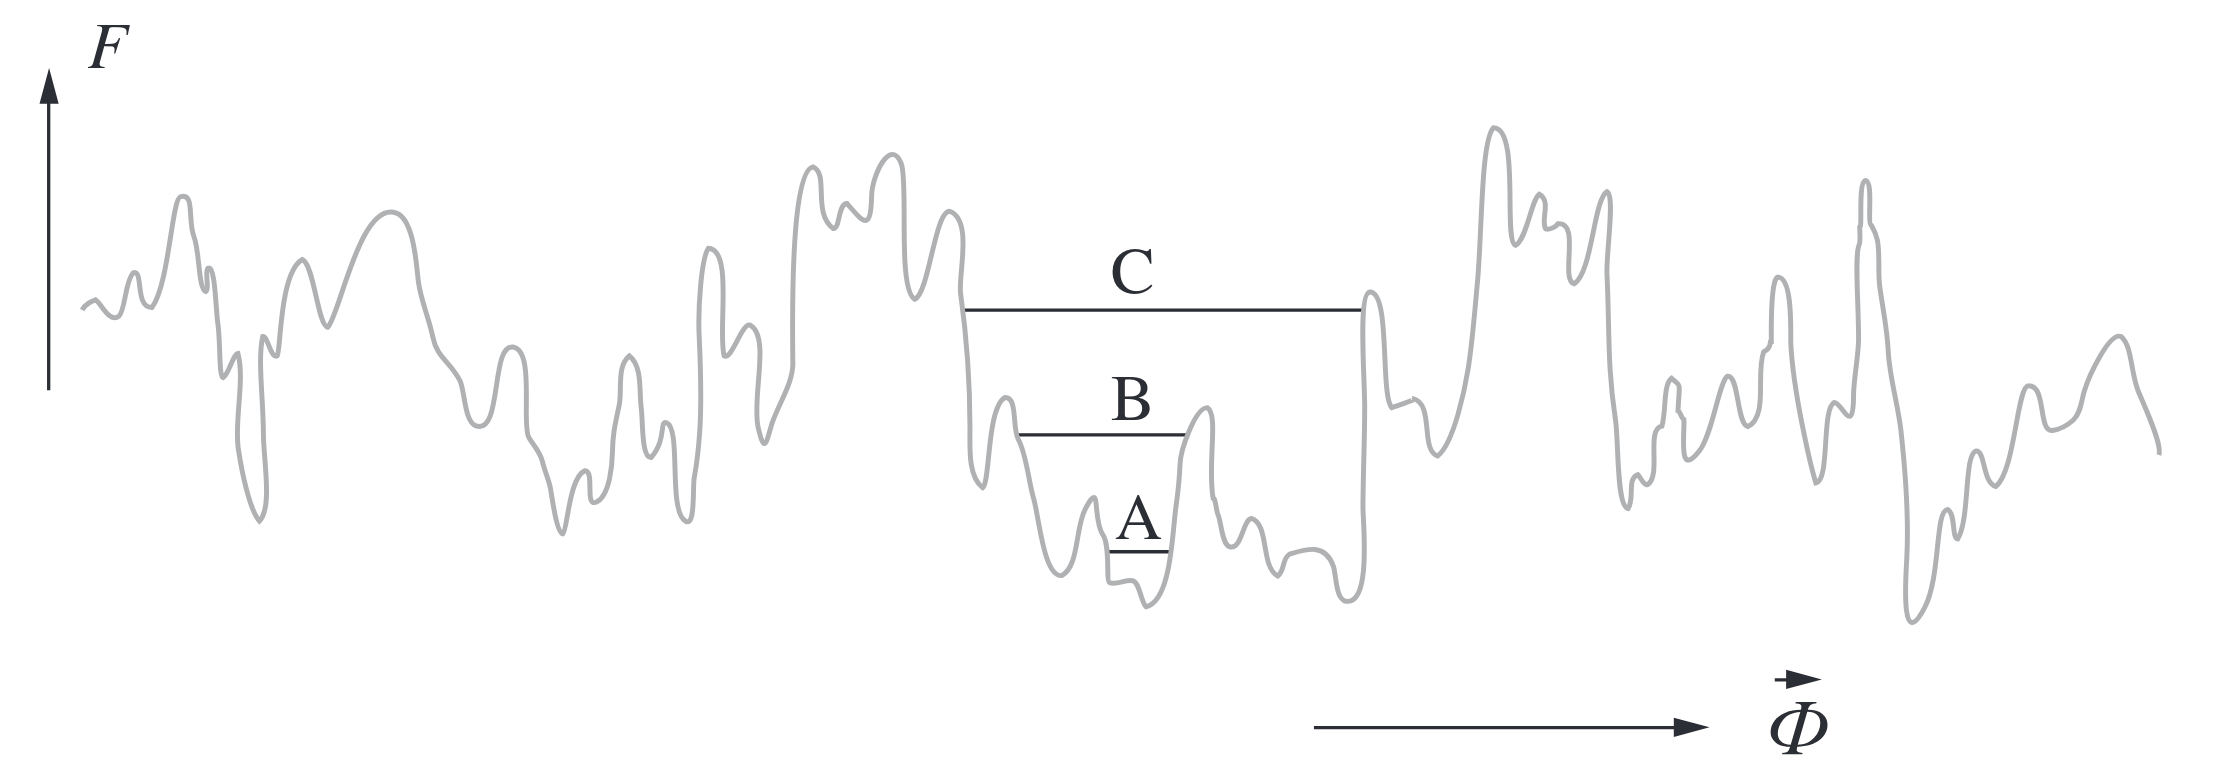
\includegraphics[width=0.9\textwidth]{Figures/spin-glass-rugged-energy-landscape.png}
%     \caption[Un exemple de paysage énergétique d'un système de verre de spin. Les multiples minimums locaux font en sorte que les algorithmes prennent du temps à résoudre le probléme. Image tirée de~\cite{}.]{Un exemple de paysage énergétique d'un système de verre de spin. Les multiples minimums locaux font en sorte que les algorithmes prennent du temps à résoudre le probléme. Image tirée de~\cite{stein2013spin}.}
%     \label{fig:spin-glass-rugged-energy-landscape}
% \end{figure}

Un contre-exemple connu de la difficulté de résolution d'un problème avec les verres de spin est le modèle $p$-spin, expliqué plus en profondeur dans la section~\ref{sec:p-spin} qui suit.
Ce modèle, quoique plus simple que les autres décrits dans cette section, possède lui aussi un paysage énergétique accidenté dans un certain régime de paramètres, mais sa résolution se fait tout de même facilement.

\section{Le modèle \texorpdfstring{$p$}{p}-spin} \label{sec:p-spin}
Le modèle $p$-spin est une variante du modèle général des verres de spins dans lequel seulement les $p$ plus proches voisins (des spins d'Ising) interagissent ensemble~\cite{}.
% de manière ferromagnétique ou antiferromagnétique.
De par sa simplicité et sa structure, un système $p$-spin se représente aisément de manière visuelle en utilisant un \emph{graphe}, terme défini à la définition~\ref{def:graph}.
\begin{definition}\label{def:graph}
    Un \textbf{graphe} $G = (V, E)$ correspond à un ensemble de sommets $V$ et d'arêtes $E$, où $E = \{uv\ |\ u, v \in V\}$. Afin de visualiser ce concept, un graphe possédant six sommets  et sept arêtes est représenté à la figure~\ref{fig:random-graph}.
\end{definition}
\begin{figure}[h]
    \centering
    \includegraphics[width=0.6\textwidth]{Figures/graph_example.pdf}
    \caption[Graphe contenant six sommets et sept arêtes.]{Graphe contenant six sommets $V = \{v_1, v_2, v_3, v_4, v_5, v_6\}$ et sept arêtes $E = \{v_1v_6, v_2v_3, v_2v_6, v_3v_4, v_3v_5, v_4v_5, v_5v_6\}$.}
    \label{fig:random-graph}
\end{figure}
En effet, ce modèle peut se modéliser par un graphe $G = (U, V, E)$ où $U$ correspond à l'ensemble de sommets qui représentent les $|U| = n$ spins, $V$ correspond à l'ensemble de sommets qui représentent les $|V| = m$ termes d'interaction et $E$ correspond à l'ensemble d'arêtes qui connectent les sommets de $U$ avec $V$.
La définition de l'ensemble $E$ fait en sorte que les sommets en $U$ ne se connectent qu'avec ceux qui se trouvent en $V$, et vice-versa, ce qui revient à dire qu'il est un graphe \emph{biparti}.
Cette représentation permet la définition suivante de l'Hamiltonien pour ce modèle:
% Le modèle $p$-spin est entièrement défini par l'Hamiltonien $\mathcal{H}$ suivant:
\begin{equation} \label{eq:ham_p-spin}
    \mathcal{H} = \frac{1}{2} \left[m -\sum_{v \in V} J_{v}\prod_{u \in N(v)} \sigma_{u} \right],
\end{equation}
où $J_v \in \left\{\pm1\right\}$ correspond au couplage des $p$ interactions au sommet $v$, $\sigma_u \in \left\{\pm1\right\}$ est le spin présent au sommet $u$ et $N(v) \subset U$ est l'ensemble des $p$ spins qui interagissent ensemble au sommet $v$.
Ce système contient donc des spins d'Ising qui interagissent de manière ferromagnétique ou antiferromagnétique avec la même intensité partout.
L'étude principale de cet Hamiltonien dans ce projet revient à << simplement >> \emph{compter} le nombre de configurations de spins $\sigma_u$ qui donnent une énergie nulle au système pour un ensemble donné de graphes.
En d'autres mots, cela revient à évaluer la \emph{fonction de partition} $Z$ à température nulle de ces systèmes.
% \begin{definition}\label{def:partition-function}
%     En mécanique statistique, la \textbf{fonction de partition} est une fonction qui décrit les propriétés statistiques d'un système dans son état d'équilibre thermodynamique. Elle est une fonction qui additionne tous les états possibles d'un système, fournissant une mesure du poids statistique de ces états.
% \end{definition}
% L'énergie totale d'un système de ce type de problème peut s'écrire comme suit:
% \begin{equation}\label{eq:p-spin_energy}
%     E(\vec{\sigma}) = \sum_{v \in V} E(\vec{\sigma}_{\{N(v)\}}),
% \end{equation}
% ce qui permet de définir la fonction de partition de la manière suivante:
% \begin{equation}\label{eq:p-spin_partition-fn}
%     Z = \sum_{\vec{\sigma}} e^{-\beta E(\vec{\sigma})} = \sum_{\vec{\sigma}} \prod_{v \in V}e^{-\beta E(\vec{\sigma}_{\{N(v)\}})}.
% \end{equation}
% Cette expression sera utile plus tard dans la définition de ce problème en réseau de tenseurs.

À toute fin pratique, il est possible de réécrire l'Hamiltonien de l'équation~\ref{eq:ham_p-spin} en définissant les termes de couplage et de spins d'une autre manière.
Comme les valeurs que les spins peuvent prendre se trouvent dans l'ensemble $\{\pm 1\}$, on peut introduire des variables \emph{booléennes} --- $b_v$ et $x_u$ ---, de la manière suivante:
\begin{equation}\label{eq:new_ham_p-spin1}
    \begin{split}
        \mathcal{H} &= \frac{1}{2} \left[m -\sum_{v \in V} (-1)^{b_v}\prod_{u \in N(v)} (-1)^{x_u} \right] = \frac{1}{2} \left[m -\sum_{v \in V} (-1)^{b_v + \sum_{u \in N(v)} x_u} \right],
    \end{split}
\end{equation}
où les termes de couplage et les spins sont redéfinis comme étant respectivement $J_v = (-1)^{b_v}$ et $x_u = (-1)^{x_u}$.
Ce changement de variable correspond simplement à faire la conversion entre les valeurs $\pm 1$ et l'ensemble $\{0, 1\}$.
Comme ces nouvelles variables sont booléennes, on ne s'intéresse qu'à la parité de l'exposant de $-1$, ce qui nous permet de finalement définir cet Hamiltonien comme suit:
\begin{equation} \label{eq:new_ham_p-spin2}
    \mathcal{H} = \frac{1}{2} \left[m -\sum_{v \in V} (-1)^{b_v + \sum_{u \in N(v)} x_u\mod{2}} \right].
\end{equation}
Avec cette nouvelle expression de $\mathcal{H}$, trouver une des configuration de spins $\vec{\sigma}$ qui mène à l'énergie minimale du système revient à résoudre l'équation suivante:
\begin{equation}
    \begin{split}
        b_v + \sum_{u \in N(v)} x_u = 0 &\mod{2}\ \forall v \in V,\\
        \implies b_v = \sum_{u \in N(v)} x_u &\mod{2}\ \forall v \in V.
    \end{split}
\end{equation}
Cette nouvelle expression à résoudre peut directement se traduire comme le système d'équations linéaires suivant:
\begin{equation} \label{eq:Bx=b}
    B\vec{x} = \vec{b} \mod 2,
\end{equation}
où $B \in \{0, 1\}^{m \times n}$ est la \emph{matrice de biadjacence} du graphe biparti $G$ qui modélise le problème initial, $\vec{x} \in \left\{ 0,1 \right\}^n$ encode la configuration des $n$ spins et $\vec{b} \in \left\{ 0,1 \right\}^m$ encode les $m$ couplages.
Les éléments de la matrice de biadjacence se définissent comme suit:
\begin{equation}\label{eq:biadjacency-matrix}
    B_{vu} = 
    \begin{cases}
            1, & \text{si $u \in N(v)$,}\\
            0, & \text{sinon.}
    \end{cases}
\end{equation}
On a donc que si un spin $\sigma_u$ interagit avec ceux qui sont dans $N(v)$ (que $B_{vu} = 1$) une arête se trouve entre le terme d'interaction $v$ et ce même spin dans $G$.

Déterminer les configurations de spins qui minimisent l'énergie de ce type de système revient à résoudre l'équation matricielle~\ref{eq:Bx=b} et compter le nombre de ces configurations revient à faire d'autres manipulations sur cette même expression.
Ces autres manipulations correspondent à convertir ce problème sous la forme de problème de \emph{satisfiabilité booléenne} (SAT), plus précisément le \#$p$-XORSAT dans le cas du modèle $p$-spin.
Ces termes sont définis dans le chapitre~\ref{ch:SAT}.



\chapter{Satisfiabilité booléenne} \label{ch:SAT}
% \lettrine{U}{n} problème d'optimisation tel que l'optimisation de horaires pour les envols et les attrissages d'avions, le problème sac-à-dos ou même le problème du voyageur de commerce sont des problèmes d'optimisation utilisés dans la vie de tous les jours.
% Ces problèmes ont tous une similarité, il est possible de les résoudre en utilisant le concept de la satisfiabilité booléenne, mais ils sont difficiles à résoudre.
% C'est pourquoi 

\section{Définition}\label{sec:def-SAT}
Dans sa forme la plus générale, un problème SAT consiste à déterminer si une formule logique, construite à l'aide d'un ensemble de variables booléennes $\vec{x} = (x_1, x_2, ..., x_n)$ et des opérateurs de conjonction ($\wedge$), de disjonction ($\vee$) et de négation ($\neg$), peut être rendue vraie, c'est-à-dire, si elle est \textit{satisfiable}~\cite{garey1979computers}.
Le problème SAT se caractérise toujours par une conjonction de \emph{clauses} qui sont elles-mêmes des disjonctions de variables sur lesquelles l'opération de négation peut être appliquée.

% Afin de mieux visualiser ce type de problème, voici un exemple aléatoire avec $n = 4$ variables et $m = 2$ clauses:
Afin de mieux visualiser et comprendre ce type de problème, un exemple aléatoire avec $n = 4$ variables et $m = 2$ clauses est donné à l'équation~\ref{eq:SAT-example}.
\begin{equation}\label{eq:SAT-example}
    \phi(\vec{x}) = (x_0 \vee \neg x_2 \vee x_3) \wedge (x_1 \vee x_2).
\end{equation}
Essayons maintenant de déterminer une solution qui satisfait ce problème.
Cela peut se faire en utilisant une approche exhaustive où on regarde chacune des combinaisons possibles pour ces clauses.
Pour la clause $c_0 = x_0 \vee \neg x_2 \vee x_3$, cette analyse est faite dans le tableau~\ref{table:c1} et la même est faite pour $c_1 = x_1 \vee x_2$ dans le tableau~\ref{table:c2}.
% \begin{table}[h]
%     \centering
%     \begin{tabular}{|c c c||c|}
%         \hline
%         $x_1$ & $x_3$ & $x_4$ & $x_1 \vee x_3 \vee x_4$ \\
%         \hline
%         0 & 0 & 0 & 0 \\
%         \hline
%         0 & 0 & 1 & 1 \\
%         \hline
%         0 & 1 & 0 & 1 \\
%         \hline
%         0 & 1 & 1 & 1 \\
%         \hline
%         1 & 0 & 0 & 1 \\
%         \hline
%         1 & 0 & 1 & 1 \\
%         \hline
%         1 & 1 & 0 & 1 \\
%         \hline
%         1 & 1 & 1 & 1 \\
%         \hline
%     \end{tabular}
%     \caption{Toutes les combinaisons de variables possibles pour la clause $c_1$.}
%     \label{table:c1}
% \end{table}
% \begin{table}[h]
%     \centering
%     \begin{tabular}{|c c||c|}
%         \hline
%         $x_2$ & $x_3$ & $x_2 \vee x_3$ \\
%         \hline
%         0 & 0 & 0\\
%         \hline
%         0 & 1 & 1\\
%         \hline
%         1 & 0 & 1\\
%         \hline
%         1 & 1 & 1\\
%         \hline
%     \end{tabular}
%     \caption{Toutes les combinaisons de variables possibles pour la clause $c_2$.}
%     \label{table:c2}
% \end{table}
\begin{table}[h]
    \parbox{.48\linewidth}{
        \centering
        \begin{tabular}{|c c c c||c|}
            \hline
            $x_0$ & $x_2$ & $\neg x_2$ & $x_3$ & $x_0 \vee \neg x_2 \vee x_3$ \\
            \hline
            0 & 0 & 1 & 0 & 1 \\
            \hline
            0 & 0 & 1 & 1 & 1 \\
            \hline
            0 & 1 & 0 & 0 & 0 \\
            \hline
            0 & 1 & 0 & 1 & 1 \\
            \hline
            1 & 0 & 1 & 0 & 1 \\
            \hline
            1 & 0 & 1 & 1 & 1 \\
            \hline
            1 & 1 & 0 & 0 & 1 \\
            \hline
            1 & 1 & 0 & 1 & 1 \\
            \hline
        \end{tabular}
        \caption{Toutes les combinaisons de variables possibles pour la clause $c_0$.}
        \label{table:c1}
    }
    \hfill
    % \hspace{0.001\textwidth}
    \parbox{.48\linewidth}{
        \centering
        \begin{tabular}{|c c||c|}
            \hline
            $x_1$ & $x_2$ & $x_1 \vee x_2$ \\
            \hline
            0 & 0 & 0\\
            \hline
            0 & 1 & 1\\
            \hline
            1 & 0 & 1\\
            \hline
            1 & 1 & 1\\
            \hline
        \end{tabular}
        \caption{Toutes les combinaisons de variables possibles pour la clause $c_1$.}
        \label{table:c2}
    }
\end{table}
Une solution pour $\phi(\vec{x})$ en est une pour laquelle $c_0$ et $c_1$ sont satisfaites en même temps.
Avec ces deux énumérations de toutes les possibilités de configurations des variables dans les clauses, il est facile de voir que la configuration $\vec{x} = (0, 1, 0, 0)$ en est une qui satisfait les deux clauses en même temps, donc le problème.
L'utilisation de cette méthode est simple dans ce cas puisque $n$ est petit, mais lorsque le nombre de variables augmente, elle devient impossible à utiliser.
En effet, si $\phi(\vec{x})$ contient $n$ variables alors il y a $2^n$ configurations possibles pour les variables.
Cela signifie que pour un grand $n$, il devient impossible de faire ce type de recherche exhaustive.

Le problème SAT a été le premier problème démontré comme appartenant à la classe de complexité \textbf{NP-complète} par Stephen Cook~\cite{cook1971}.
% --------- Début du nouvellement ajouté -----------------
Avant de définir cette classe de complexité, il est important de comprendre que les problèmes se séparent, d'après les connaissances d'aujourd'hui~\cite{millenniumPrizeProblems}, en deux; les problèmes dits \emph{faciles} (\textbf{P}) et ceux qui sont \emph{difficiles} (\textbf{NP}).
Ceux qui sont facilement résolvable sont ceux qui sont dans la classe \textbf{P}, soient tous les problèmes de décision qui sont solvables dans un temps polynomial.
Ceux qui sont difficiles se retrouvent dans la classe \textbf{NP} (\textit{nondeterministic polynomial time} en anglais), donc tous les problèmes de décision pour lesquels la solution peut se faire vérifier facilement (dans un temps polynomial).
Avec cela, on peut maintenant définir la classe \textbf{NP-complète} comme suit:
% --------- Fin du nouvellement ajouté -------------------
% Cette classe de complexité contient deux points importants: elle regroupe des problèmes qui font parties de la classe de complexité \emph{NP} et elle est \emph{complète}.
% Les définitions de ces deux classes de complexité se retrouvent respectivement aux définitions~\ref{def:NP} et~\ref{def:NP-complete}.
% Pour ces deux catégories, tout problème qui s'y trouve est un problème pour lequel il est facile de vérifier si une solution est bonne, mais difficile de trouver cette dite solution.
% La hiérarchie de ces classes de complexité est montrée dans la figure~\ref{fig:complexites}, où on voit aussi les classes \emph{P} et \emph{NP-difficile} , toutes deux définies respectivement aux définitions~\ref{def:P} et~\ref{def:NP-hard}.
% \begin{definition}\label{def:P}
%     La classe de complexité \textbf{P} contient tous les problèmes de décision qui sont solvables facilement (dans un temps polynomial).
% \end{definition}
% \begin{definition}\label{def:NP}
%     La classe de complexité \textbf{NP} (<< nondeterministic polynomial time >> en anglais) contient tous les problèmes de décision pour lesquels la solution peut se faire vérifier rapidement (dans un temps polynomial).
% \end{definition}
\begin{definition}\label{def:NP-complete}
    % La classe de complexité \textbf{NP-complet} est une classe qui englobe tous les problèmes $A$ dans NP pour lesquels il est possible de réduire tout autre problème NP $B$ à $A$ facilement (en temps polynomial).
    La classe de complexité \textbf{NP-complète} est une classe des problèmes \textbf{NP} auxquels tous les autres problèmes dans \textbf{NP} peuvent être réduits en temps polynomial.
\end{definition}
On retrouve ensuite la classe de complexité \textbf{\#P}, qui rassemblent les problèmes qui ont comme objectif de \emph{compter} le nombre de solution(s) de problèmes dans \textbf{NP} qui les satisfont.
Il y a aussi la classe \textbf{\#P-complète}, qui englobe tous les problèmes se retrouvant dans \textbf{\#P} pour lesquels il est possible de réduire tout autre problème de cette classe à ceux-ci facilement (en temps polynomial).
Les problèmes qui s'y retrouvent sont tous au moins aussi difficiles que ceux qui sont dans la classe \textbf{NP-complète}.
% \begin{definition}\label{def:NP-hard}
%     La classe de complexité \textbf{NP-difficile} contient les problèmes qui sont au moins aussi difficiles que ceux se trouvant dans la classe NP-complet, sans toutefois se limiter aux problèmes de décision.
% \end{definition}
Finalement, dans la hiérarchie des classes de complexité montrée à la figure~\ref{fig:complexites}, on retrouve la classe \textbf{NP-difficile}. 
Celle-ci englobe tous les problèmes qui sont au moins aussi difficiles que ceux se trouvant dans la classe \textbf{NP-complète}, sans toutefois se limiter aux problèmes de décision.
\begin{figure}[h]
    \centering
    % ajouter figure de la hiérarchie des classes de complexités de P à NP-difficile
    \includegraphics[width=0.6\textwidth]{Figures/complexity_classes_hierarchy.pdf}
    \caption[Schéma de la hiérarchie des classes de complexité.]{Schéma de la hiérarchie des classes de complexité (en supposant que P~$\ne$~NP).}
    \label{fig:complexites}
\end{figure}

% Les deux autres classes de complexités qui n'ont pas été définies plus haut, mais qui se trouvent dans la figure~\ref{fig:complexites}, sont \emph{\#P} et \emph{\#P-complet}, définies respectivement aux définitions~\ref{def:sharp-P} et~\ref{def:sharp-P-complete} ci-dessous.
% Celles-ci englobent les problèmes pour lesquels l'objectif est de compter le nombre de solution satisfaisant le problème initial.
% Un exemple de problème de ce type est \#SAT, le problème pour lequel l'objectif est de déterminer le nombre de configurations de variables qui satisfont un problème donné.
% \begin{definition}\label{def:sharp-P}
%     La classe de complexité \textbf{\#P} comprend les problèmes de comptage liés aux problèmes de décision présents dans NP.
%     Plus précisément, un problème appartient à \#P s'il consiste à compter le nombre de solutions qui satisfont un problème donné de la classe NP.
% \end{definition}
% \begin{definition}\label{def:sharp-P-complete}
%     La classe de complexité \textbf{\#P-complet} est une classe qui englobe tous les problèmes $A$ dans \#P pour lesquels il est possible de réduire tout autre problème \#P $B$ à $A$ facilement (en temps polynomial).
%     Les problèmes dans \#P-complet sont au moins aussi difficiles que ceux se trouvant dans NP-complet.
% \end{definition}


% Ces types de problèmes ne sont pas seulement des problèmes purement théoriques, puisqu'ils peuvent être utillisés dans notre vie de tous les jours.
% Certains exmples concrets sont le \emph{problème de voyageur de commerce} et le \emph{problème du sac à dos}.
% Le premier est un problème dans lequel un voyageur de commerce souhaite trouver un chemin qui va le faire passer par les $N$ villes (destinations) dans lesquelles il doit y faire une livraison sans y repasser par la suite tout en minimisant le coût (la distance parcourue) de ce voyage.
% Ce problème se retrouve par exemple dans l'optimisation des chemins pour les camionneurs ou pour les livreurs.
% Le second est un problème dans lequel, par exemple, une personne souhaite partir en randonnée et veut optimiser sons sac à dos au niveau de la nourriture.
% Elle souhaite minimiser le poids de cette nourriture tout en maximisant ses apports nutritifs.

En ajoutant une contrainte stipulant que chacune des clauses d'un problème SAT possède exactement $k$ variables, on se retrouve à étudier le problème $k$-SAT qui est, lui aussi, dans la catégorie de complexité \textbf{NP-complète}.
Compter le nombre de solution(s) satisfaisant ce type de problème correspond au problème \#$k$-SAT et lui aussi se retrouve dans la catégorie de complexité \textbf{\#P-complète}, pour toutes les valeurs de $k \geq 2$~\cite{valiant_complexity_1979}.

Le problème $k$-SAT possède plusieurs variantes, comme \textit{$1$-in-$3$} SAT et \textit{not-all-equal} 3-SAT (NAE3-SAT), et la plupart se retrouvent dans la même classe de complexité que celui-ci.
De plus, chacune d'elle peut se caractériser par le paramètre $\alpha \equiv m / n$, la densité de clauses.
Ce paramètre est relié au phénomène de transition de phase dans ces problèmes.
Pour le problème de type $k$-SAT, ce phénomène se produit à une certaine valeur du paramètre $\alpha$ où la probabilité que le problème soit solvable passe drastiquement de $1$ vers $0$.
Dans le cas du problème $k$-SAT avec $k = 3$, la transition est montrée dans la figure~\ref{fig:SAT_phase-transition}.
\begin{figure}[h]
    \centering
    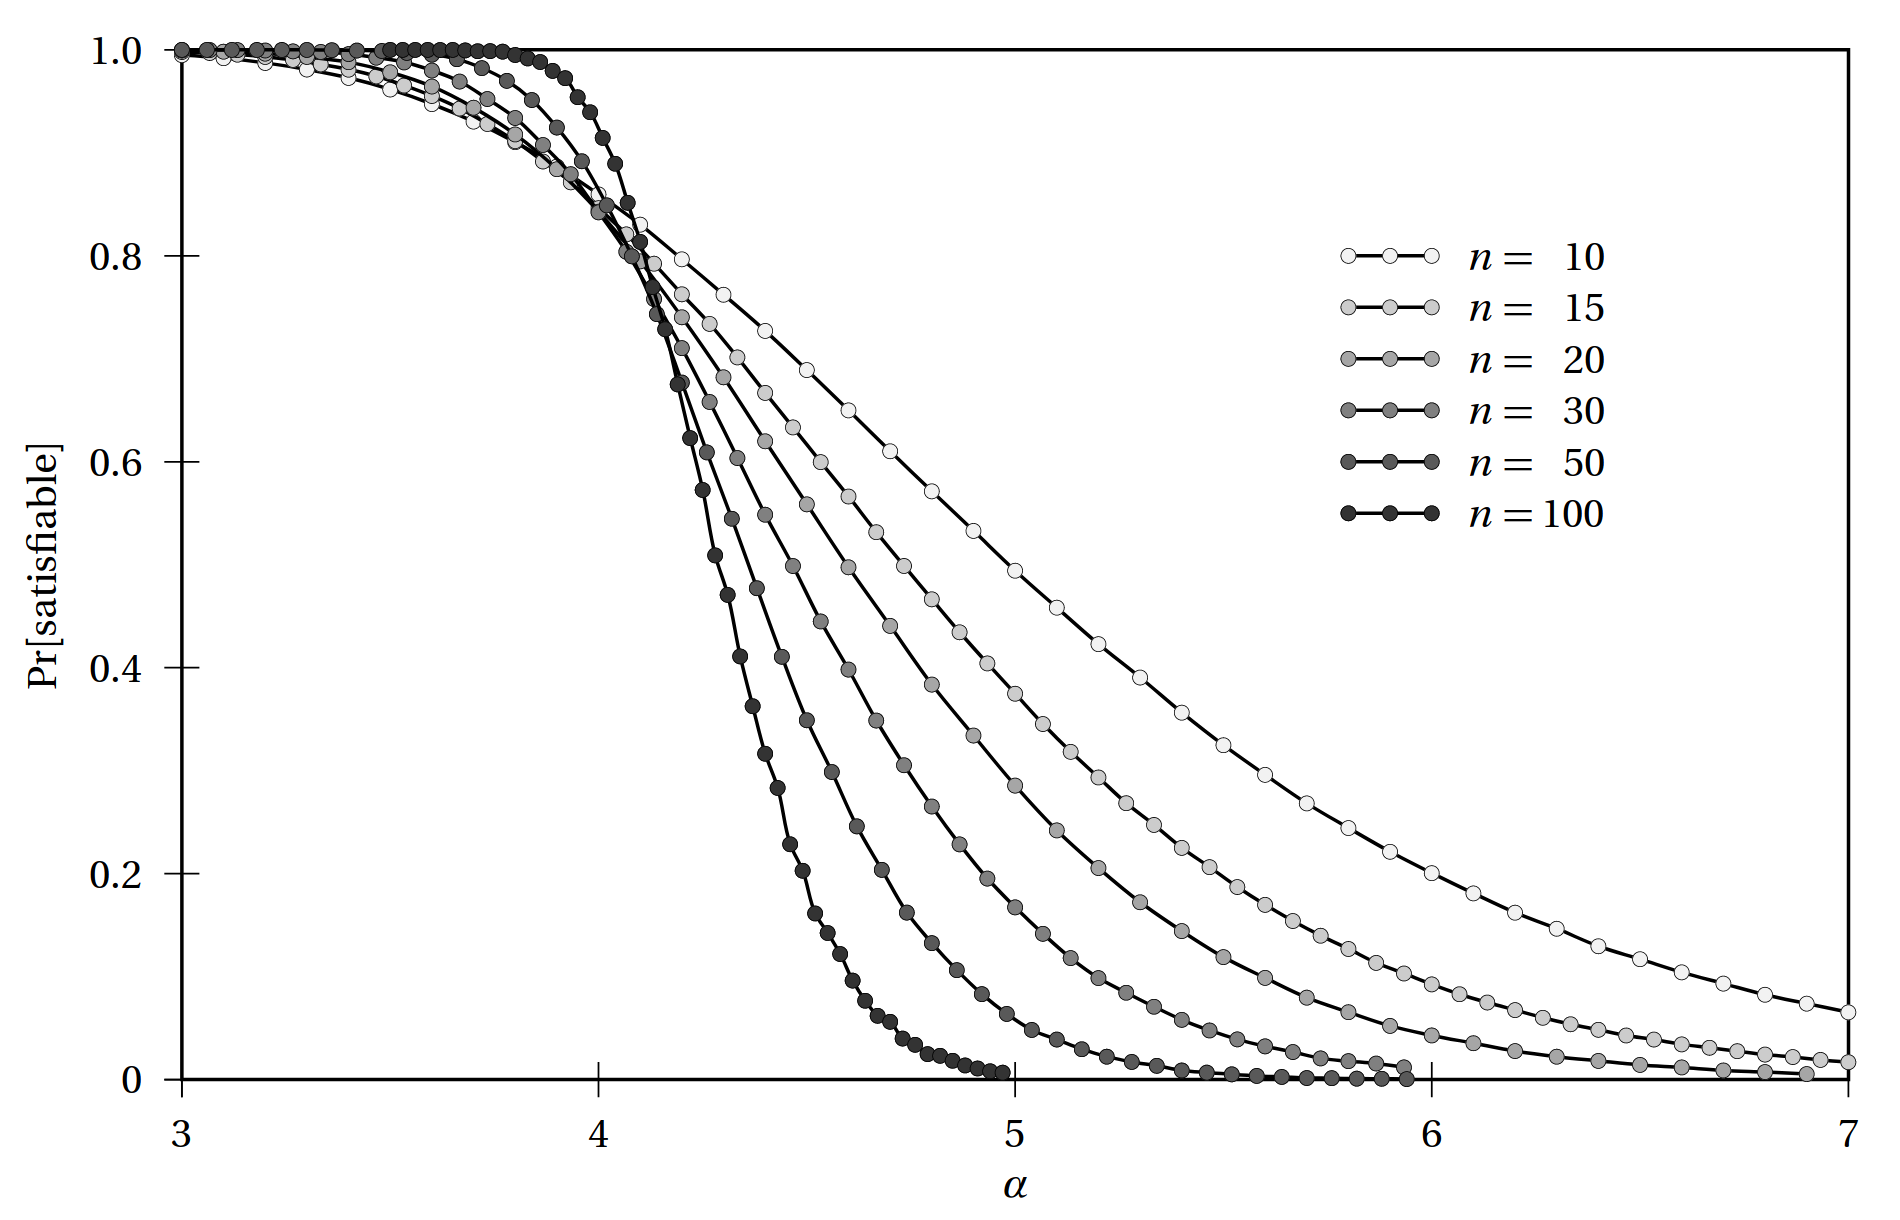
\includegraphics[width=0.7\textwidth]{Figures/SAT_phase-transition.png}
    \caption[La probabilité de satisfaction d'un problème $3$-SAT en fonction de la densité de clauses $\alpha$.]{La probabilité de satisfaction d'un problème $3$-SAT en fonction de la densité de clauses $\alpha$. On voit que plus le nombre de variables $n$ augmente, plus la chute devient abrupte. En fait, si on traçait la courbe dans la limite thermodynamique ($n \rightarrow \infty$), il y aurait un passage instantané de 1 vers 0 à $\alpha = \alpha_c$. Image tirée de \emph{The Nature of Computation}~\protect\cite{moore_nature_2011}.}
    \label{fig:SAT_phase-transition}
\end{figure}
Comme on peut le voir dans cette figure, le problème $3$-SAT passe de \textit{satisfiable} à \textit{non-satisfiable} à $\alpha \approx 4.267$~\cite{moore_nature_2011}.
On appelle cette transition: la transition de phase SAT-UNSAT.

Maintenant que la notion de problème SAT est définie, on peut s'attaquer au problème qui modélise le modèle de $p$-spin définit à l'équation~\ref{eq:Bx=b}.
Ce problème est, comme mentionné à la fin de la section~\ref{sec:p-spin}, $p$-XORSAT, qui est défini dans la section~\ref{sec:k-xorsat}.


\section{Le problème \#\texorpdfstring{$k$}{k}-XORSAT}\label{sec:k-xorsat}
Le problème $k$-XORSAT est le problème principal dans ce mémoire dans le cadre de l'analyse du problème $p$-spin.
Afin de relier les deux, il suffit de poser $k = p$ et de respecter les encodages mentionnés après l'équation~\ref{eq:Bx=b}, et la conversion est faite.
La présentation du problème général dans cette section est faite en utilisant seulement $k$, la variable $p$ sera utilisée plus tard dans le chapitre~\ref{ch:tns-and-p-xorsat}.

Ce problème ne requiert qu'une seule modification des opérateurs dans les clauses par rapport au problème standard $k$-SAT.
L'opérateur de disjonction y est remplacé par l'opérateur de sommation modulo $2$ ($\oplus$), qui se fera nommer << sommation booléenne >> au travers de ce mémoire puisque les variables qui se retrouvent dans les problèmes analysés sont booléennes.
Avec la matrice de biadjacence $B$ et le vecteur $\vec{b}$ de l'équation~\ref{eq:Bx=b}, on peut définir une instance $\phi(\vec{x})$ du problème $k$-XORSAT de la manière suivante:
\begin{equation}\label{eq:xorsat_def}
    \begin{split}
        \phi(\vec{x}) &= \bigwedge_{v = 0}^{m - 1} c_v \text{, avec }m = \alpha n,\\
        c_v &= 1 \oplus b_v \oplus B_v \cdot \vec{x},\\
        \vec{x} &= \left(x_1, x_2, \ldots, x_n \right) \in \{0, 1\}^n,
    \end{split}
\end{equation}
où $B_v \in \{0, 1\}^n$ est la ligne $v$ de la matrice $B$, $b_v$ indique l'élément $v$ du vecteur $\vec{b}$ et $B_v \cdot \vec{x}$ indique la sommation booléenne des variables présentent dans la clause $c_v$.
Les éléments de $\vec{b}$ peuvent aussi être vus comme étant les parités requises pour satisfaire chacune des clauses du problème.
Lorsque $c_v = 1$, ce qui se produit lorsque $b_v \oplus B_v \cdot \vec{x} = 0$, on dit que la clause est \emph{satisfaite}.

Comme mentionné dans la section~\ref{sec:def-SAT}, lorsqu'on génère ces types d'instances de manière complètement aléatoire, on a que le paramètre de densité de clause $\alpha$ caractérise en grande partie le problème.
Pour le problème $k$-XORSAT en particulier, celui-ci contient deux transitions de phases~\cite{mezard_alternative_2002}.
La première se produit à $\alpha_d$, qui indique une transition \emph{dynamique} dans la structure de l'espace des solutions de manière à séparer (en distance de Hamming) les solutions en plusieurs \emph{grappes}.
La seconde se produit à la transition critique $\alpha_c$ où, avec une probabilité élevée, une instance devient non-satisfiable.
Celle-ci est conceptuellement équivalente à la transition de phase SAT/UNSAT montrée dans la figure~\ref{fig:SAT_phase-transition}.
Ce point montre une transition de phase similaire même lorsque $\vec{b} = \vec{0}$, ce qui signifie que $\vec{x} = \vec{0}$ est toujours une solution possible~\cite{ricci2001simplest}.
Afin de mieux comprendre les effets qu'a ce paramètre sur l'espace des solutions mentionnée pour $\alpha_d$, son évolution en fonction de $\alpha$ est schématisée à la figure~\ref{fig:solution-space}.
\begin{figure}[h]
    \centering
    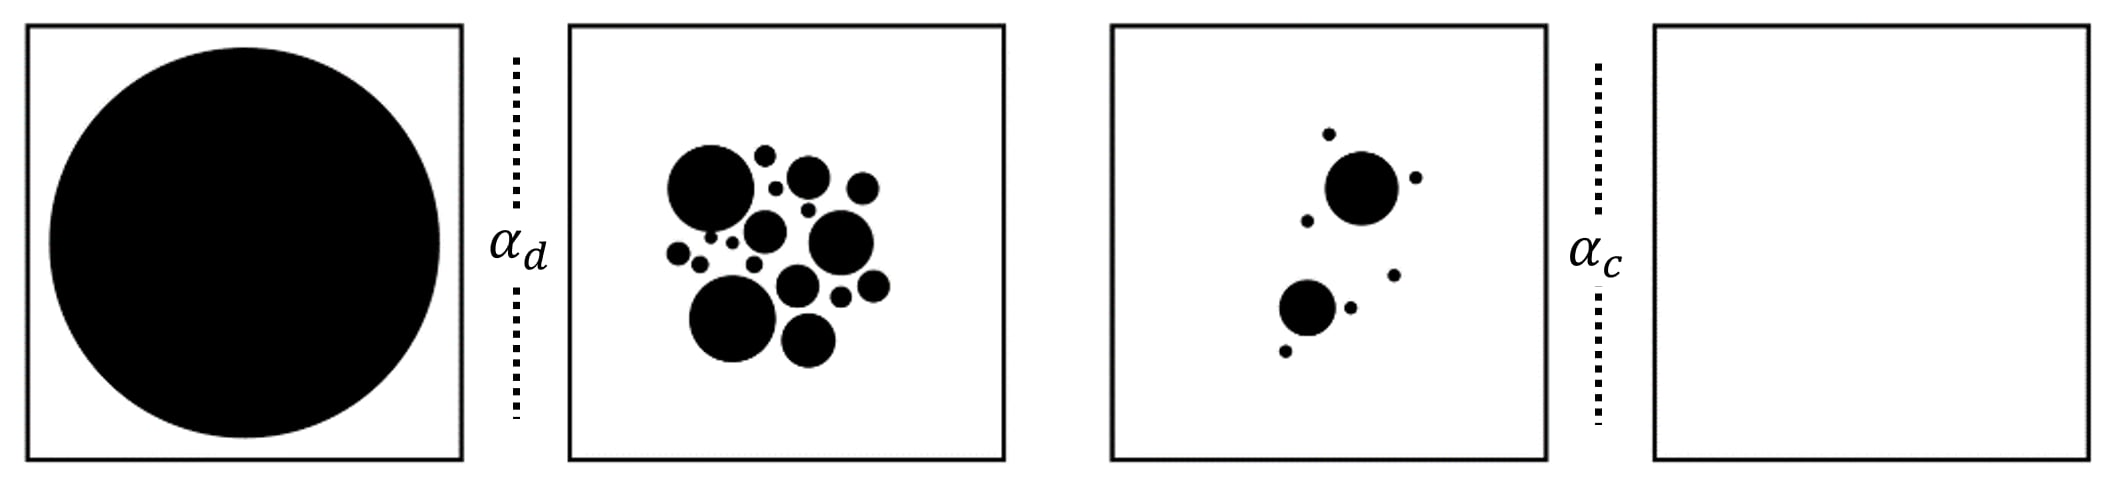
\includegraphics[width=0.77\textwidth]{Figures/solution_space_evolution.jpeg}
    \caption[L'évolution de l'espace des solutions pour le problème \mbox{$k$-XORSAT}.]{Schéma de l'évolution de l'espace des solutions pour le problème \mbox{$k$-XORSAT}. Image tirée de~\protect\cite{moore_nature_2011}.}
    \label{fig:solution-space}
\end{figure}
Dans le cas de $3$-XORSAT, ces deux paramètres sont $\alpha_d \approx 0.818$ et $\alpha_c \approx 0.918$~\cite{mezard_alternative_2002}.
De plus, comparativement aux autres variantes du problème \#$k$-SAT, le problème \#$k$-XORSAT ne se retrouve pas dans la classe de complexité \textbf{\#P-complète}, mais bien dans \textbf{P}, donc on sait qu'il est facile de le résoudre.
Ce point sera plus développé dans la section~\ref{subsec:GE}.

De nombreux algorithmes ont été adaptés afin d'être applicables sur le problème $k$-XORSAT, tels que le recuit quantique adiabatique~\cite{patil_obstacles_2019}, l'élimination gaussienne~\cite{braunstein_complexity_2002} et l'algorithme d'élimination de feuilles~\cite{mezard_alternative_2002} pour en nommer quelques-uns.
% un algorithme adiabatique quantique~\cite{farhi2000quantum}.
Dans les prochaines sections, on va commencer par définir l'algorithme utilisant l'élimination gaussienne (section~\ref{subsec:GE}) pour ensuite définir celui d'élimination de feuilles, une méthode graphique qui élimine la redondance dans le problème (section~\ref{subsec:leaf-removal-algorithm}) et on finit par définir une méthode graphique connue pour simplifier un problème donné (section~\ref{subsec:XORSAT-simplifications}).

% DON'T USE THIS
% Ce n'est pas par hasard que ce même $p$ se retrouve dans le nom de ces deux problèmes, car cette variable correspond directement à la même valeur dans les deux cas.
% En effet, avoir $p$ spins qui interagissent ensemble revient à avoir $p$ variables dans chacune des clauses du problème de satisfiabilité.

\subsection{Élimination gaussienne}\label{subsec:GE}
Étant donnée une instance $\phi(\vec{x})$ du problème $k$-XORSAT contenant $m$ clauses et $n$ variables, on commence par la traduire sous la forme de la matrice de biadjacence $B$ de l'équation~\ref{eq:Bx=b}.
Il est aussi nécessaire d'avoir les parités de chacune des clauses afin de pouvoir utiliser $\vec{b}$.
Par la suite, on applique l'élimination gaussienne sur la matrice augmentée $[B|\vec{b}]$, où toutes les opérations sont modulo deux.
Une fois cette étape terminée, si on retrouve au moins une inconsistance dans le système, il n'existe aucune solution pouvant satisfaire ce problème.
Cette inconsistance vient du fait qu'une ligne aurait la forme $[0\ 0\ \dots 0 | 1]$, ce qui n'a aucun sens puisque la somme modulo $2$ de plusieurs variables ayant un poids nul ne peut jamais être égale à un.
Toutefois, si ces inconsistances ne sont pas présentes, alors le nombre de solutions satisfaisant le problème donné est:
\begin{equation}\label{eq:nb_sols_ge}
    \text{\#Solutions} = 2^{n - \mathrm{rang}(B)}.
\end{equation}

Dans~\cite{braunstein_complexity_2002}, les auteurs ont étudié les complexités en temps et en mémoire de l'élimination gaussienne pour la résolution du problème \#$k$-XORSAT avec $k = 3$ en utilisant une version de cet algorithme qu'ils définissent comme étant << simple >>.
Cette version résout les équations linéaires présentes dans l'équation~\ref{eq:Bx=b} dans l'ordre dans laquelle elles apparaissent déjà.
Ils y montrent que cet algorithme simple résout le problème donné avec une complexité en temps et en mémoire proportionnelle à $n$ pour $\alpha \leq 2/3$.
Lorsque ce paramètre dépasse le seuil de $2/3$, les complexités en temps et en mémoire deviennent respectivement $\propto n^3$ et $\propto n^2$.
Les auteurs ont également présenté une version << intelligente >> de cet algorithme, dans laquelle les variables qui apparaissent dans le moins d'équations sont abordées en premier (en cas d'égalité, elles sont choisies arbitrairement).
On résout ensuite pour cette variable et on la substitue dans les équations restantes.
Ils font valoir que cette version plus intelligente résout le problème avec des ressources (le temps et la mémoire) proportionnelles à $n$ lorsque $\alpha < \alpha_d$.
Lorsque $\alpha > \alpha_d$, ces ressources passent respectivement à $\propto n^3$ et $\propto n^2$.

Ces changements de complexité pour ces deux versions de l'algorithme sont dus au fait que chaque étape de l'élimination gaussienne peut introduire de nouveaux $1$s dans $B$, augmentant ainsi leur densité en fonction du nombre d'éléments dans cette matrice.
Cette augmentation est suffisante pour modifier ces complexités, car la matrice ne reste pas creuse comme on peut le voir avec l'exemple donné dans la figure~\ref{fig:GE-ones-density}.
\begin{figure}[h]
    \centering
    \includegraphics[width=0.9\textwidth]{Figures/matrice.pdf}
    \caption[Évolution de la densité de 1s lors de l'élimination gaussienne avec $n = m = 1024$ ($\alpha = 1$).]{Évolution de la densité de 1s lors de l'élimination gaussienne avec $n = m = 1024$ ($\alpha = 1$). Les points noir et blanc correspondent respectivement aux 0s et aux 1s dans la matrice et $t$ représente le pourcentage de complétion de l'algorithme. Image tirée de~\protect\cite{braunstein_complexity_2002}.}
    \label{fig:GE-ones-density}
\end{figure}


Lorsqu'on résout une équation qui contient une variable qui n'apparaît que dans celle-ci, on peut interpréter graphiquement le processus comme un algorithme d'\emph{élimination des feuilles}, décrit dans la section~\ref{subsec:leaf-removal-algorithm} suivante.
Cet algorithme donne une intuition quant à la raison pour laquelle la version << intelligente >> de l'élimination gaussienne est plus efficace et aidera à expliquer le comportement de l'algorithme développé dans le cadre de ce projet qui utilise les réseaux de tenseurs.
Cet algorithme est expliqué plus tard dans les sections~\ref{sec:eliminate-redundancy-with-bond-compression} et~\ref{sec:sweeping-method}.

\subsection{Algorithme d'élimination des feuilles}\label{subsec:leaf-removal-algorithm}
Supposons qu'on a une instance $k$-XORSAT avec $k = 3$ et une variable, que l'on définit comme étant $x_0$, n'apparaît que dans l'équation linéaire:
\begin{equation}\label{eq:c0-example}
    x_0 \oplus x_1 \oplus x_2 = b_0,
\end{equation}
qui correspond à la clause $c_0$ dans le problème.
Peu importe les valeurs que les variables $x_1$ et $x_2$ prennent, il est toujours possible de choisir $x_0$ de manière à satisfaire cette clause en la fixant à:
\begin{equation}\label{eq:x0-value}
    x_0 = x_1 \oplus x_2 \oplus b_0.
\end{equation}
En sachant cela, on peut enlever cette clause du problème initial, le résoudre, et définir la valeur de $x_0$ en fonction des deux autres variables à la fin.
% On a donc que satisfaire l'équation~\ref{eq:x0-value} permet de donner une configuration de variables qui satisfait le problème donné si et seulement si le problème simpifié est satisfiable. % du problème simplifié
Cependant, une fois que cette clause est retirée du problème, il se peut que $x_1$ et/ou $x_2$ ne se retrouvent que dans une seule équation/une seule clause.
On peut donc retirer cette seconde clause contenant la variable n'apparaissant qu'une seule fois dans le problème modifié.
Ce processus se répète jusqu'à ce que toutes les variables qui restent soient présentes au moins deux fois dans le problème simplifié.
En termes de la matrice de biadjacence dans l'équation~\ref{eq:Bx=b}, chaque colonne va contenir au moins deux $1$s.
Il est à noter que si une instance dépend de $n$ variables et que seulement $n - q$ de ces variables se retrouvent dans le problème, alors on peut simplement ignorer ces $q$ variables manquantes et multiplier le nombre de solutions satisfaisant le problème par $2^q$.
% sait qu'elles peuvent prendre n'importe quelle valeur et satisfaire le problème.
Cet algorithme se nomme élimination des feuilles~\cite{mezard_alternative_2002, cocco_rigorous_2003} et il permet le simplifier grandement un problème $k$-XORSAT.

Les étapes décrites ici se visualisent bien sur un graphe qui modélise le problème.
Pour un problème de type $k$-XORSAT, c'est un graphe biparti où on retrouve deux types de sommets; les sommets << clause >> et les sommets << variable >>.
Ce graphe est entièrement décrit par la matrice de biadjacence $B$ de l'équation~\ref{eq:Bx=b}.
Comme $B \in \mathbb{R}^{m \times n}$, ce graphe contiendra exactement $m$ sommets << clause >> et $n$ sommets << variable >>.
De plus, si $B_{vu} = 1$, on retrouve une arête entre le sommet << clause >> $c_v$ et le sommet << variable >> $x_u$.
On se retrouve donc avec des sommets dont les \emph{degrés} --- le nombre d'arêtes qui lui sont connectées dans le graphe --- respectent l'équation~\ref{eq:vs_degrees}.
% (terme défini à la définition~\ref{def:degree})
% \begin{definition}\label{def:degree}
%     Le \textbf{degré} d'un sommet $v$ est le nombre d'arêtes qui lui sont connectées dans le graphe. Ainsi, si ce sommet est connecté à $q$ arêtes, on écrit $\mathrm{deg}(v) = q$.
% \end{definition}
% Dans la théorie des graphes, le degré d'un sommet $v$ est le nombre d'arêtes qui lui sont connectées dans le graphe.
Ainsi, si ce sommet est connecté à $q$ arêtes, on écrit $\mathrm{deg}(v) = q$.
\begin{equation}\label{eq:vs_degrees}
    \mathrm{deg}(s) = \begin{cases}
        k & \text{, si } s \in V,\\
        \sum_{v \in V}B_{vs} & \text{, si } s \in U.
    \end{cases}
\end{equation}

Graphiquement, l'algorithme débute avec un graphe biparti $G$ qui représente le problème, puis il trouve, de manière itérative, des sommets variables $u \in U$ pour lesquels $\mathrm{deg}(u) = 1$.
Une fois qu'un sommet qui respecte ce degré est trouvé, l'algorithme élimine le sommet clause $v$ qui lui est connecté ainsi que toutes les arêtes qui lui sont associées.
En appliquant ces étapes jusqu'à ce qu'il soit impossible de les appliquer, on se retrouve avec deux conclusions possibles:
\begin{enumerate}
    \item Toutes les arêtes se sont fait enlever par le processus.
    \item Il reste des variables de degré deux et plus, laissant donc un \emph{noyau} du graphe initial.
\end{enumerate}
Dans le premier cas, on dit que l'algorithme d'élimination de feuilles a simplifié le problème en entier.
Dans le second, le noyau restant est encore un problème de type $k$-XORSAT, mais simplifié dans lequel toutes les variables restantes sont présentes au moins deux fois dans les clauses restantes.
Une fois que ce noyau est résolu, on peut déterminer une solution du problème initial en évaluant les valeurs des variables qui ont été simplifiées par l'algorithme puisqu'elles dépendent de celles qui sont dans le noyau. 

Dans~\cite{mezard_alternative_2002}, les auteurs montrent que, dans la limite thermodynamique ($n \rightarrow \infty$), l'algorithme d'élimination des feuilles réussi à réduire le graphe correspondant au graphe complètement simplifié lorsque $ \alpha < \alpha_d$ pour l'ensemble dans lequel $p = 3$ et où toutes les clauses sont choisies uniformément au hasard.
Comme on peut fixer un sommet variable de degré $1$ à une valeur à chaque étape de cet algorithme afin d'éliminer un sommet clause et ses arêtes, le nombre de solutions satisfaisant un problème $k$-XORSAT donné pour lequel il ne reste pas de noyau est de $2^{n-m}$, où $m$ est le nombre de clauses du problème et $n$ est le nombre de variables.
Lorsque $\alpha > \alpha_d$, un noyau du graphe va rester après l'application de l'algorithme d'élimination des feuilles.
Cela signifie que cet algorithme à lui seul ne peut pas résoudre ce problème en entier.
Le paramètre $\alpha = \alpha_d$ correspond à une transition dynamique dans ce problème et il correspond aussi à un changement dans la structure de l'ensemble des solutions du problème, comme mentionné dans la section~\ref{sec:k-xorsat}.
La version << intelligente >> de l'élimination gaussienne utilise ce principe pour obtenir une amélioration face à la version << simple >>.

% EST-CE QUE JE FAIS CE PARAGRAPHE ???
% We also note that when no core remains at the end of leaf removal, one can interpret the algorithm as finding a permutation of the rows and columns of the matrix $A$ such that one can transform $A$ into triangular form. Suppose the variable $x_i$ only appears in equation $j$. One would then permute the rows $1$ and $j$ of $A$, as well as the columns $1$ and $i$. Ignoring the first row and column of $A$, repeat the same procedure. Continuing in this way will yield a matrix $A'$ which is in triangular form and has the same rank as $A$. The triangular form of $A'$ implies that its rank is simply the number of rows, allowing one to calculate the number of solutions.

Dans le cas du problème $k$-XORSAT, cet algorithme démontre qu'il est possible d'identifier et d'éliminer graphiquement un certain type de redondance, réduisant ainsi la taille du problème en se concentrant seulement sur le noyau restant.
Graphiquement, cette redondance reliée aux variables de degré $1$ n'est pas la seule qui se retrouve dans ce problème; deux autres sont expliquées dans la section~\ref{subsec:XORSAT-simplifications} suivante.

\subsection{Simplifications graphiques connues} \label{subsec:XORSAT-simplifications}
Comme mentionné dans la section précédente, certaines règles graphiques permettant de simplifier le problème $k$-XORSAT sont déjà connues.
Deux de ces règles sont la loi de \emph{bialgèbre} et la loi d'\emph{Hopf}~\cite{kasselQuantumGroups1995, denny_algebraically_2012}.
Analyser ces règles sera utile pour la compréhension du fonctionnement interne de l'algorithme développé dans le cadre de ce mémoire.
Ici, l'analyse est faite pour $\vec{b} = \vec{0}$.

La loi d'Hopf stipule que si une variable est présente deux fois dans une seule clause d'un problème de type XORSAT, alors elle n'est pas nécessaire puisque son information est redondante.
Cette loi est représentée dans la figure~\ref{fig:hopf-law} ci-dessous.
\begin{figure}[h]
    \centering
    \includegraphics[width=0.7\textwidth]{Figures/hopf_law.pdf}
    \caption[Représentation graphique de la loi de Hopf.]{Représentation graphique de la loi de Hopf. Les sommets de type << clause >> sont représentés par des carrés bleus et les sommets de type << variable >> sont représentés par des cercles verts.}
    \label{fig:hopf-law}
\end{figure}
Il est facile de voir que cette règle est vraie dans le cas des problèmes XORSAT puisque les variables et les sommations sont booléennes dans les clauses.
Ainsi, on a que $x_0 \oplus x_0 \oplus x_1 = x_1$, où $x_0$ ne sert à rien dans la représentation du problème.

La loi de bialgèbre permet de simplifier les cas où on retrouve deux sommets << clauses >> qui sont tous les deux connectés à deux sommets << variables >>.
La simplification est moins directe que celle de la loi d'Hopf, mais commençons par analyser son impact sur l'ensemble de quatre sommets décrits précédemment dans la figure~\ref{fig:bialgebra-law}.
\begin{figure}[h]
    \centering
    \includegraphics[width=0.7\textwidth]{Figures/bialgebra_law.pdf}
    \caption[Représentation graphique de la loi de bialgèbre.]{Représentation graphique de la loi de bialgèbre. Les sommets de types << clause >> sont représentés par des carrés bleus et les sommets de type << variable >> sont représentés par des cercles verts.}
    \label{fig:bialgebra-law}
\end{figure}
Cette structure permet de simplifier cet ensemble en seulement une variable et une clause.
La simplification vient du fait que les deux clauses intiales sont:
\begin{equation}
    \begin{split}
        c_0 &= x_0 \oplus x_1 \oplus x_2,\\
        c_1 &= x_0 \oplus x_1 \oplus x_3.
    \end{split}
\end{equation}
Comme l'objectif est de satisfaire ces deux clauses en même temps, on se retrouve avec $x_k  = x_l$ puisque $x_0$ et $x_1$ sont présentes et interagissent de la même manière dans ces deux clauses.
On peut donc considérer que $x_2$ et $x_3$ sont une seule et unique variable $x$.
Avec le fait que ces deux clauses contiennent les même variables, elles sont équivalentes à avoir une seule clause $c$ qui contient $x_0$, $x_1$ et $x$.
Le changement de côté des deux types de sommets dans la figure~\ref{fig:bialgebra-law} vient du fait que $c$ contient les même variables $x_0$ et $x_1$ que précédemment et du fait que $x = x_2 = x_3$.

Comme on peut le voir, certaines simplifications graphiques sont possibles à effectuer avec un problème de type XORSAT.
Ces simplifications correspondent à l'éliination de redondances qui sont présentes dans le problème initial, alors trouver un moyen de les simplifier de manière automatique pourrait être un atout pour la résolution du problème.
Dans ce mémoire, on utilise les réseaux de tenseurs, définis au chapitre~\ref{ch:TN} ci-dessous, ainsi que certaines méthodes qui leurs sont reliées afin de trouver et éliminer ces redondances automatiquement.

% % --------------Réseaux de tenseurs------------------------



\chapter{Réseaux de tenseurs}\label{ch:TN}
% \lettrine{L}{'algèbre} linéaire est une branche des mathématiques qui a permis de développer des outils et des techniques fondamentaux pour résoudre des systèmes d'équations linéaires, analyser des transformations linéaires et comprendre la structure des espaces vectoriels.
% Ces concepts sont essentiels dans de nombreux domaines, comme l'ingénierie, la physique et l'informatique pour en nommer quelques-uns.
% Les réseaux de tenseurs en sont une branche qui se trouve aujourd'hui à la pointe des méthodes de calcul modernes et qui sont utilisés dans de nombreux domaines.
% Ils sont, par exemple, particulièrement importants pour la simulation classique des circuits quantiques.

\section{Définition}\label{sec:tn-definition}
D'un point de vue strictement d'algèbre linéaire, les réseaux de tenseurs correspondent à une structure qui encode une liste de multiplications de \emph{tenseurs}.
%, défini à la définition~\ref{def:tensor}.
\begin{definition}\label{def:tensor}
    Un \textbf{tenseur} est un objet algébrique permettant de généraliser les concepts de scalaires (tenseurs de rang-$0$), de vecteurs (tenseurs de rang-$1$) et de matrices (tenseurs de rang-$2$) à des dimensions plus élevées.
    Ces trois premiers cas et leur généralisation sont montrés dans la figure~\ref{fig:tensor-schematic-def} dans le formalisme des réseaux de tenseurs.
    Finalement, un tenseur de rang-$d$ se note:~$T_{i_0 i_1 \cdots i_{d-1}}$, où les $i$ sont les indices de chacune des dimensions de $T$.
    \begin{figure}[h]
        \centering
        \begin{subfigure}{.245\textwidth}
            \centering
            \includegraphics[width=.95\linewidth]{Figures/degree0-tensor.pdf}
            \caption{}
            \label{fig:tensor-scalar}
        \end{subfigure}
        \begin{subfigure}{.245\textwidth}%[width=0.24\textwidth]{}
            \centering
            \includegraphics[width=.95\linewidth]{Figures/degree1-tensor.pdf}
            \caption{}
            \label{fig:tensor-vector}
        \end{subfigure}
        \begin{subfigure}{.245\textwidth}%[width=0.24\textwidth]{}
            \centering
            \includegraphics[width=.95\linewidth]{Figures/degree2-tensor.pdf}
            \caption{}
            \label{fig:tensor-matrix}
        \end{subfigure}
        \begin{subfigure}{.245\textwidth}%[width=0.24\textwidth]{}
            \centering
            \includegraphics[width=.95\linewidth]{Figures/degreed-tensor.pdf}
            \caption{}
            \label{fig:tensor-tensor}
        \end{subfigure}
        \caption{Représentation schématique d'un tenseur pour \textbf{(a)} un scalaire, \textbf{(b)} un vecteur, \textbf{(c)} une matrice et \textbf{(d)} un tenseur de rang-$d$.}
        \label{fig:tensor-schematic-def}
    \end{figure}
\end{definition}

Intuitivement, on peut imaginer un réseau de tenseurs comme un graphe dans lequel chaque sommet représente un tenseur et où chaque arête représente les dimensions communes sur lesquelles deux tenseurs vont se multiplier.
Il est possible pour un tenseur dans ce réseau d'être connecté à une arête qui n'est connectée à aucun autre tenseur, ce qui signifie simplement que cette dimension du tenseur ne subit aucune multiplication.
En contractant ensemble les tenseurs voisins --- multiplier ces tenseurs sur leurs dimensions communes --- il est possible d'évaluer efficacement une multitude de quantités, ce qui fait de ce concept une méthode numérique très utile.
Développé à l'origine pour l'évaluation efficace de valeurs moyennes en mécanique quantique et l'étude de systèmes à $N$ corps~\cite{white1992density, schollwock2011density}, cet outil numérique possède aujourd'hui des applications dans plusieurs domaines tels que la simulation de circuits quantiques~\cite{huang_classical_2020, seitz_simulating_2023}, l'intelligence artificielle~\cite{pmlr-v130-miller21a, wang_tensor_2023} et la science de l'information~\cite{cichocki2016tensor} pour en nommer quelques-uns.
Ils peuvent également être utilisés pour résoudre les problèmes $k$-SAT et compter le nombre de solutions qu'ils possèdent~\cite{garcia-saez_exact_2011, liu2021tropical}.
Dans le cadre de ce mémoire, contracter l'entièreté des tenseurs dans un réseau modélisant un problème $k$-XORSAT donnera le nombre de solutions qui le satisfont.
Ce point est plus développé dans le chapitre~\ref{ch:tns-and-p-xorsat}, où le lien entre les trois chapitres de la partie théorique est fait.

Ci-dessous, les principales idées des méthodes reliées aux réseaux de tenseurs sont définies.
Ces méthodes sont: la contraction (section ~\ref{sec:contraction}), l'ordre de contraction (section ~\ref{sec:contraction-ordering}) ainsi que la compression de lien (section ~\ref{sec:compression}).


\section{La contraction} \label{sec:contraction}
% A single tensor is a multidimensional array of values.
Comme mentionné dans la section~\ref{sec:tn-definition}, le concept de contraction dans le domaine des réseaux de tenseurs correspond à la multiplication de deux tenseurs voisins sur leurs dimensions communes.
On dit aussi que cette multiplication se produit sur les indices qu'ils partagent, à cause de la notation des tenseurs se trouvant dans un réseau de tenseurs.
Graphiquement, le nombre d'axes (ou le \emph{rang}) d'un tenseur est équivalent au degré du sommet qui lui correspond dans le graphe.
La \emph{taille} d'un tenseur --- le nombre d'éléments qu'il contient --- est le produit des dimensions de ces axes.
La taille d'un réseau de tenseurs correspond alors à la somme des tailles de tous les tenseurs qui s'y trouvent.
Pour tout algorithme utilisant un réseau de tenseurs, on doit suivre la taille de ce réseau afin de s'assurer que celle-ci ne dépasse pas les ressources disponibles d'un ordinateur en mémoire.
Plus particulièrement, on doit considérer comment la contraction des tenseurs peut modifier la taille du réseau.

Un exemple simple de contraction est la multiplication matrice-vecteur, qui est graphiquement représentée dans la figure~\ref{fig:tn_mat-vec_multiplication}.
\begin{figure}[h]
    \centering
    \includegraphics[width=0.7\textwidth]{Figures/tn_matrix_vector_multiplication.pdf}
    \caption{Multiplication matrice-vecteur dans le formalisme des réseaux de tenseurs.}
    \label{fig:tn_mat-vec_multiplication}
\end{figure}
Le vecteur $\vec{u}$, un tenseur de rang-$1$, est représenté par un sommet avec une seule arête qui lui est connectée et la matrice $M$, un tenseur de rang-$2$, est aussi un sommet, mais avec deux arêtes.
La multiplication matrice-vecteur montrée à la figure~\ref{fig:tn_mat-vec_multiplication} peut aussi s'écrire comme la sommation suivante:
\begin{equation}\label{eq:einsum}
    \sum_j M_{ij}u_j = v_i.
\end{equation}
De manière générale, on peut écrire la contraction complète d'un réseau de tenseurs comme une sommation sur tous les indices communs.
Dans le formalisme des réseaux de tenseurs, deux tenseurs ayant des dimensions communes sont appelés \emph{voisins}.

Lorsqu'on fait la contraction de tenseurs où les axes communs ont la même dimension, il est possible de déterminer graphiquement la dimension résultante simplement en regardant le rang du nouveau sommet.
Dans la figure~\ref{fig:tn_mat-vec_multiplication}, le tenseur final est de rang-$1$, ce qui est le même que le rang du vecteur $\vec{u}$.
Dans d'autres situations, la taille de ce tenseur contracté peut être plus élevée que les tenseurs originaux.
En effet, supposons que l'on contracte deux tenseurs de rangs $d_1$ et $d_2$ qui partagent un seul indice et que tous les dimensions de ces tenseurs sont de dimension 2.
La taille du tenseur contracté sera de $2^{d_1 + d_2 - 2}$, donc elle évolue de manière exponentielle avec les rangs des tenseurs.
Cette croissance exponentielle est le point qui rend la contraction complète d'un réseau de tenseurs numériquement difficile, alors il est important de déterminer un ordre de contraction judicieux.


\section{L'ordre de contraction}\label{sec:contraction-ordering}
Techniquement, il est possible d'effectuer la contraction complète d'un réseau de tenseurs dans n'importe quel ordre.
Par contre, l'ordre choisi a le potentiel de grandement faire varier la taille du réseau de tenseurs durant les contractions intermédiaires.
Idéalement, cet ordre va minimiser la taille du réseau de tenseurs, limitant ainsi les ressources en mémoire nécessaires dans un ordinateur.
Cela fait en sorte que la contraction complète a plus de chance d'être faisable.

Étant donné un ordre de contraction et des tenseurs possédant tous des axes de dimension $d$, on peut définir la \emph{largeur de contraction} $W$ (concept défini à la définition~\ref{def:contraction-width}) du réseau~\cite{gray_hyper-optimized_2021} de deux manières équivalentes:
\begin{equation} \label{eq:contraction-width}
    W =
    \begin{cases}
        \max_{v \in P} \mathrm{deg}(v) & \text{(graphiquement)},\\
        \max_{T \in \mathcal{T}} \log_d{s(T)} & \text{(tenseurs)}.\\
    \end{cases}
\end{equation}
\begin{definition}\label{def:contraction-width}
    La \textbf{largeur de contraction} correspond au nombre maximal de dimensions/d'indices qu'un tenseur a atteints durant la contraction d'un réseau de tenseurs.
\end{definition}
Dans la représentation graphique, $P$ est l'ensemble de sommets représentant les tenseurs présents à toutes les étapes de la contraction.
Dans la représentation tensorielle, $\mathcal{T}$ est l'ensemble de tous les tenseurs qui sont présents à toutes les étapes de la contraction et $s(T)$ est la taille du tenseur $T$.
Il est à noter ici que $W$ dépend de l'ordre dans laquelle la contraction du réseau de tenseurs est faite.
Par la suite, $2^W$ --- la taille maximale atteinte par un tenseur durant la contraction --- capture les besoins en mémoire pour l'ensemble de la contraction à un préfacteur prêt~\cite{gray_hyper-optimized_2021}.

Déterminer un ordre de contraction est un problème d'optimisation en soit et des algorithmes existent pour en trouver un qui est optimisé en fonction de la structure du réseau de tenseurs.
Dans certains cas, comme un réseau de tenseurs en forme de grille carrée, déterminer l'ordre optimal est facile tandis que dans d'autres, comme un réseau de tenseurs aléatoires, c'est beaucoup plus fastidieux~\cite{gray_hyper-optimized_2022}.
Afin de montrer l'importance de cet ordre de contraction, analysons son impact sur le réseau de tenseurs en forme d'échelle longue de $N$ tenseurs représenté à la figure~\ref{fig:latter-tn}.
\begin{figure}[h]
    \centering
    \includegraphics[width=0.6\textwidth]{Figures/latter_tn.pdf}
    \caption{Réseau de tenseurs en forme d'échelle.}
    \label{fig:latter-tn}
\end{figure}
Cet exemple montre particulièrement bien l'importance d'un bon ordre de contraction puisque dans un cas, il est impossible de le contracter tandis que dans un autre, c'est très simple.
Ces deux cas sont montrés dans la figure~\ref{fig:latter-tn-good-contraction-cases}.
\begin{figure}[h]
    \centering
    \begin{subfigure}{.47\textwidth}
        \centering
        \includegraphics[width=0.95\linewidth]{Figures/latter_tn_bad_contraction_order.pdf}
        \caption{On contracte tous les tenseurs du haut (ordre en bleu). On se retrouve ensuite avec un tenseur de rang-$N$ (encerclé en rouge) qui a potentiellement une taille beaucoup trop élevé (donc un problème au niveau de la mémoire d'un ordinateur).}
        \label{fig:latter-tn-bad-contraction-order}
    \end{subfigure}
    % \hfill
    \hspace{0.02\textwidth}
    \begin{subfigure}{.47\textwidth}
        \centering
        \includegraphics[width=.95\linewidth]{Figures/latter_tn_good_contraction_order.pdf}
        \caption{On contracte tous les tenseurs de haut en bas (ordre en bleu), ce qui mène vers des tenseurs qui ont un rang maximal de $4$. On contracte ensuite de gauche à droite (ordre en vert) et on obtient la contraction complète du réseau.}
        \label{fig:latter-tn-good-contraction-order}
    \end{subfigure}
    \caption{L'analyse schématique de l'importance de l'ordre de contraction pour un réseau de tenseurs en forme d'échelle long de $N$ tenseurs.}
    \label{fig:latter-tn-good-contraction-cases}
\end{figure}

De manière générale, les ressources nécessaires (en temps et en mémoire) pour complètement contracter un réseau de tenseurs augmentent de manière exponentielle avec le nombre de tenseurs, ce qui signifie que c'est un problème difficile, voire impossible lorsqu'ils sont présents en grand nombre.
Malgré cela, une méthode appelée la \emph{compression de lien}, méthode expliquée dans la section suivante, permet de pousser ces limites en acceptant le fait que le résultat final soit approximé.


\section{La compression de lien}\label{sec:compression}
Dans sa forme la plus simple, la compression de lien consiste à effectuer une opération de \emph{contraction-décomposition} sur des tenseurs voisins au sein d'un réseau de tenseurs.
Le terme << lien >> réfère à un indice commun entre deux tenseurs.
L'étape de décomposition utilise principalement des méthodes de révélation de rang telles que QR et la décomposition en valeurs singulières (ou \textit{SVD} venant de l'anglais \textit{Singular Value Decomposition}).
Avant de définir le processus de compression de lien (section~\ref{subsec:bond-compression}), ces deux types de décompositions sont expliqués à la section~\ref{subsec:QR-and-SVD}.
% définissions d'abord les outils qui lui sont nécessaires, comme les types de \emph{décompositions matricielles} ainsi que le \emph{remodelage de tenseurs}.

\subsection{Décomposition matricielle}\label{subsec:QR-and-SVD}
La décomposition QR décompose, comme son nom le laisse présager, une matrice $M \in \mathbb{R}^{m \times n}$ en deux matrices $Q \in \mathbb{R}^{m \times r}$ et $R \in \mathbb{R}^{r \times n}$, où $r$ est le rang de $M$ (son nombre de lignes linéairement indépendantes).
Les matrices $Q$ et $R$ correspondent respectivement à une matrice orthogonale et à une matrice triangulaire supérieure.

Quant à elle, la SVD est similaire à la décomposition en valeurs propres, mais pour les matrices qui peuvent aussi être rectangulaires.
Celle-ci décompose une matrice $M \in \mathbb{C}^{m \times n}$ en trois matrices $U \in \mathbb{C}^{m \times r}$, $\Sigma \in \mathbb{C}^{r \times r}$ et $V^\dagger \in \mathbb{C}^{r \times n}$.
Les matrices $U$ et $V$ sont des matrices orthonormales et $\Sigma$ est une matrice carrée diagonale contenant les valeurs singulières ($\sigma$) de $M$ placées en ordre décroissant.
% L'impacts de la SVD est schématiquement représentée dans la figure~\ref{fig:matrix-decompositions}.
% \begin{figure}
%     \centering
%     \includegraphics[width=0.8\textwidth]{Figures/}
%     \caption{Visualisation graphique de l'application de la SVD sur une matrice $M$.}
%     \label{fig:SVD-illustration}
% \end{figure}
De ces deux méthodes, la SVD joue un rôle crucial dans certains algorithmes de réseaux de tenseurs comme l'état en produit de matrices (ou \textit{MPS} venant de l'anglais \textit{Matrix Product State})~\cite{hauschild2018efficient}.
De plus, cette méthode est particulièrement utile afin d'approximer des matrices puisqu'elle fournit l'accès aux valeurs singulières classées de manière décroissante.
Cela nous permet de fixer une valeur seuil sur les valeurs propres, qu'elle soit absolue ou relative, et de garder seulement celles qui y sont supérieures, ainsi que les colonnes et les lignes de $U$ et $V$ qui leur correspondent, menant à une approximation de la matrice.

L'impact de l'application de la SVD sur une matrice peut être visuellement représentée à l'aide d'une image.
Numériquement, une image contient des données pour les couleurs \textcolor{red}{rouge}, \textcolor{green}{vert} et \textcolor{blue}{bleu} qui ne sont que des matrices dont chacune des valeurs est reliée à une teinte de la couleur correspondante.
On peut donc appliquer la SVD sur ces trois matrices en ne gardant que $q$ valeurs singulières pour ensuite reconstruire l'image compressée.
Un exemple de ce processus est montré à la figure~\ref{fig:svd-on-figure}.
\begin{figure}[h]
    \centering
    \includegraphics[width=\textwidth]{Figures/quicophy_compressed.pdf}
    % \input{Figures/quicophy_compressed.pgf}
    % \caption{Le processus d'application de la SVD sur l'image de gauche. Chacun des canaux de couleurs de cette figure est représentée par une matrice de rang $280$ (elles possèdent $280$ valeurs singulières). Ces valeurs (normalisées par la plus élevée) sont toutes montrées dans le graphique au milieu pour ces trois canaux. La valeur seuil fait en sorte que seulement les $50$ premières valeurs singulières sont conservées après l'application de la SVD. La reconstruction de l'image compressée est donnée par la figure de droite.}
    \caption[Le processus de SVD appliqué sur une image.]{Le processus de SVD appliqué à l'image de gauche décompose chaque canal de couleur en une matrice de rang $280$ (correspondant à $280$ valeurs singulières). Les valeurs singulières, normalisées par rapport à la plus élevée, sont illustrées dans le graphique central pour les trois canaux. Un seuil est ensuite appliqué pour ne conserver que les $50$ premières valeurs singulières. L'image compressée résultante est présentée dans la figure de droite.}
    \label{fig:svd-on-figure}
\end{figure}
Le graphique se trouvant entre les deux figures du logo du groupe de recherche QuICoPhy montre toutes les valeurs singulières de ce logo, normalisées par la plus élevée.
On voit très bien qu'ici, beaucoup de ces valeurs singulières ont une importance minime comparativement aux premières puisque les trois courbes pour les trois canaux de couleurs tendent rapidement vers zéro.
Ainsi, appliquer une valeur seuil nous permettant de garder seulement les $50$ premières valeurs singulières permet de reconstruire une image qui est une excellente approximation de la figure initiale.
On a donc directement que cette matrice de rang $50$ est une excellente approximation de la matrice initiale.

Cette observation vient du fait que la SVD permet de faire la meilleure approximation de rang $q$ d'une matrice donnée.
En effet, selon le théorème d'Eckart-Young~\cite{eckart_approximation_1936, dax2014low}, la meilleure approximation de rang-$q$ possible pour une matrice $M = U \Sigma V^\dagger$ avec une matrice $M_q$ de rang $q$ correspond à:
% } (bien expliqué dans l'article~\cite{
\begin{equation}\label{eq:eckart-young}
    M_q = \sum_{i=0}^{q-1}\sigma_i u_i v^\dagger_i,
\end{equation}
où $q$ est le nombre de valeurs singulières conservées (le rang de $M_q$) et $u_i$ et $v_i$ sont les colonnes $i$ de $U$ et $V$ respectivement.
La SVD est donc une excellente méthode pour extraire le rang d'une matrice et en faire la meilleure approximation possible.

\subsection{Méthodes pour la compression de lien}\label{subsec:bond-compression}
La compression de lien peut se faire selon une multitude de processus.
Entre deux tenseurs voisins, la manière naïve est de les contracter et de décomposer ce nouveau tenseur avec la SVD.
Cependant, cette méthode peut potentiellement mener à des problèmes de mémoires puisque s'ils contiennent tous les deux, par exemple, $2^{31}$ éléments et qu'ils partagent deux axes de dimensions $2$, alors le tenseur contracté contiendra $2^{60}$ éléments.
Ce nombre astronomique d'éléments fait en sorte qu'il serait impossible de représenter ce tenseur avec un ordinateur.
Cependant, si on applique une recette légèrement plus complexe, cette compression de lien devient possible.

Cette recette, montrée dans la figure~\ref{fig:compression-schedule}, nécessite l'utilisation des deux décompositions matricielles expliquées dans la section~\ref{subsec:QR-and-SVD}.
\begin{figure}[h]
    \centering
    \includegraphics[width=0.7\textwidth]{Figures/compression_schedule.pdf}
    \caption{Processus de compression de lien généralement utilisé dans le domaine des réseaux de tenseurs.}
    \label{fig:compression-schedule}
\end{figure}
Comme on peut le voir, la décomposition QR est appliquée sur les deux tenseurs voisins $A$ et $B$.
À cette première étape, on peut se poser la question suivante: comment est-il possible d'appliquer la décomposition QR sur un tenseur de rang différent à $2$?
Afin de faire cela, il faut utiliser le principe de \emph{remodelage} de tenseur, montré graphiquement à la figure~\ref{fig:tensor-reshape} et bien expliqué dans~\cite{baker2021methodes}.
\begin{figure}[h]
    \centering
    \includegraphics[width=0.75\textwidth]{Figures/tensor-matricization.pdf}
    \caption[Le remodelage d'un tenseur de rang-$5$ à un tenseur de rang-$2$.]{Le remodelage d'un tenseur de rang-$5$ $T_{i_0i_1i_2i_3i_4}$ de dimensions $(2, 2, 2, 2, 2)$ en matrice $T_{ij}$ de dimensions $(8, 4)$ où les indices $i_0$, $i_1$ et $i_2$ deviennent l'indice $i$ et les deux autres deviennent l'indice $j$.}
    \label{fig:tensor-reshape}
\end{figure}
Remodeler un tenseur revient à changer le format d'un tenseur en fusionnant ou en divisant ses axes sans perdre l'information qu'il représente.
Ainsi, si on a un tenseur de rang-$3$ $T_{abc}$ dont les dimensions sont $(4,4,4)$, il nous est possible de le réécrire comme un tenseur de rang-$4$ $T_{ab'b"c}$  avec les dimensions $(4,2,2,4)$.
Dans cet exemple, l'indice $b$ de dimension $4$ a été divisé en deux indices $b'$ et $b"$ de dimensions $2$.
Il est aussi possible d'ajouter des axes triviaux (des indices triviaux) à ce tenseur, lui donnant les dimensions $(1,4,4,1,4)$ par exemple.
Dans le cas de la compression de lien, ce principe nous permet de << \textit{matriciser} >> un tenseur de n'importe quelle dimension.
Ce terme signifie simplement que tout tenseur peut se rapporter à une matrice, comme l'exemple donné à la figure~\ref{fig:tensor-reshape}.
Ainsi, l'application de la décomposition QR sur les tenseurs $A$ et $B$ de la figure~\ref{fig:compression-schedule} cache l'étape de matricisation de ces deux tenseurs.
Par la suite, On se retrouve avec les matrices $R$ des tenseurs initiaux $A$ et $B$, lesquelles se multiplient à l'étape d'après pour donner la matrice $R_{AB}$.
On applique ensuite la SVD sur cette nouvelle matrice en gardant seulement celles qui respectent la valeur seuil spécifiée initialement.
On termine par séparer les valeurs singulières ainsi que les matrices $U$ et $V^\dagger$ à gauche et à droite et on obtient finalement un lien compressé entre les tenseurs $A$ et $B$, qui sont devenus les tenseurs approximés $\tilde{A}$ et $\tilde{B}$.
On voit donc clairement pourquoi ce processus permet d'éviter le potentiel problème de la rencontre d'un tenseur de rang trop élevé, puisqu'il ne contracte pas les tenseurs voisins.
% \begin{equation}\label{eq:eckart-young}
%     ||M - B||_F \geq ||M - M_k||_F = \sum_{i=k}^{r}\sigma_i,
% \end{equation}
